% Second Review Presentation
% Compile with: pdflatex presentation.tex  (Overleaf / TeX Live / MiKTeX)

\documentclass[aspectratio=169,11pt]{beamer}

% ---------- Theme and colours ----------
\usetheme{Madrid}
\usecolortheme{default}
\definecolor{UniversityBlue}{RGB}{16,62,110}
\definecolor{AccentBlue}{RGB}{30,136,229}
\definecolor{LightBlue}{RGB}{232,242,252}
\definecolor{DarkGray}{RGB}{55,65,81}
\definecolor{GoodGreen}{RGB}{27,122,61}
\definecolor{BadRed}{RGB}{176,32,32}
\definecolor{NoiseOrange}{RGB}{230,126,34}

\setbeamercolor{structure}{fg=UniversityBlue}
\setbeamercolor{palette primary}{bg=UniversityBlue,fg=white}
\setbeamercolor{palette secondary}{bg=AccentBlue,fg=white}
\setbeamercolor{frametitle}{bg=UniversityBlue,fg=white}
\setbeamercolor{block title}{bg=UniversityBlue,fg=white}
\setbeamercolor{block body}{bg=LightBlue,fg=black}
\setbeamercolor{alerted text}{fg=AccentBlue}

% ---------- Packages ----------
\usepackage[T1]{fontenc}
\usepackage[utf8]{inputenc}
\usepackage{lmodern}
\usepackage{graphicx}
\usepackage{booktabs}
\usepackage{array}
\usepackage{tabularx}
\usepackage{tikz}
\usetikzlibrary{positioning,arrows.meta,matrix,calc}
\usepackage{pgfplots}
\pgfplotsset{compat=1.16}
\usepackage{amsmath}
\usepackage{listings}
\usepackage{xcolor}
\usepackage{colortbl}
\usepackage{hyperref}

% ---------- General settings ----------
\setbeamertemplate{navigation symbols}{}
\setbeamertemplate{caption}[numbered]
\setbeamertemplate{itemize item}{\color{AccentBlue}$\blacktriangleright$}
\setbeamertemplate{itemize subitem}{\color{UniversityBlue}$\bullet$}
\setbeamersize{text margin left=0.7cm,text margin right=0.7cm}

\setbeamertemplate{footline}{%
  \leavevmode%
  \hbox{%
    \begin{beamercolorbox}[wd=.42\paperwidth,ht=2.7ex,dp=1.1ex,leftskip=.6em]{author in head/foot}%
      \insertshorttitle
    \end{beamercolorbox}%
    \begin{beamercolorbox}[wd=.46\paperwidth,ht=2.7ex,dp=1.1ex,center]{date in head/foot}%
      Department of Computer Science and Engineering
    \end{beamercolorbox}%
    \begin{beamercolorbox}[wd=.12\paperwidth,ht=2.7ex,dp=1.1ex,center]{page number in head/foot}%
      \insertframenumber/\inserttotalframenumber
    \end{beamercolorbox}%
  }%
  \vskip0pt%
}

\lstset{
  basicstyle=\ttfamily\scriptsize,
  keywordstyle=\color{UniversityBlue}\bfseries,
  commentstyle=\color{gray},
  stringstyle=\color{AccentBlue},
  numbers=left,
  numberstyle=\tiny\color{gray},
  frame=single,
  breaklines=true,
  showstringspaces=false
}

\newcommand{\up}[1]{\textcolor{GoodGreen}{\textbf{#1}}}
\newcommand{\dn}[1]{\textcolor{BadRed}{#1}}
\tikzset{
  box/.style={draw=UniversityBlue,fill=LightBlue,rounded corners,minimum height=0.9cm,align=center,font=\small},
  qbox/.style={draw=GoodGreen,fill=green!8,rounded corners,minimum height=0.9cm,align=center,font=\small},
  nbox/.style={draw=NoiseOrange,fill=orange!12,rounded corners,minimum height=0.9cm,align=center,font=\small},
  arrow/.style={-{Stealth[length=2.4mm]},thick,draw=AccentBlue},
}

% ---------- Project details ----------
\title[GNN Initialization for VQE + QNGD]{Noise-Aware Geometry-Guided Graph Neural Initialization\\for Variational Quantum Eigensolvers}
\subtitle{Second Review}
\author[Barath, Nithyasree, Madhangi]{%
  R.K.\ Barath (3122235001029)\\
  Nithyasree.K (3122235001092)\\
  Madhangi Karimanal (3122235001073)
}
\institute[SSN College of Engineering]{%
  Guided by: Dr.\ Sneka Nandhini\\[2mm]
  Department of Computer Science and Engineering\\
  Sri Sivasubramaniya Nadar College of Engineering
}
\date{Academic Year 2026--2027}

\begin{document}

% 1. Title
\begin{frame}[plain]
  \titlepage
\end{frame}

% 2. First review
\begin{frame}{First Review -- Queries and Answers}
  \small
  \begin{block}{Q1: Run the paper's vanilla VQE under the same conditions as our method}
    \scriptsize Re-implemented VQEzy's method (Adam, $\eta=10^{-3}$, 2000 steps) on the
    \textbf{same} 158 test instances, ansatz, simulator, ground energies and \textbf{same random
    starts} as the QNGD and GNN runs; identical device-level circuit counting (parameter-shift
    cost charged). Found: VQEzy's stored runs are 1-layer, so the method was re-run, not copied.
  \end{block}
  \begin{block}{Q2: Define a proper evaluation metric}
    \scriptsize \textbf{Circuit executions to target} (within 1\% of best energy reached; also 0.05
    of exact ground) $\cdot$ \textbf{circuit reduction} vs.\ baseline
    $=1-\sum\text{cost}_{\text{method}}/\sum\text{cost}_{\text{baseline}}$ (unreached runs charged
    full budget) $\cdot$ \textbf{success rate} (how often the target is reached) $\cdot$
    \textbf{final energy gap} $\cdot$ all noiseless \emph{and} noisy.
  \end{block}
\end{frame}

% 3. Problem statement
\begin{frame}{Problem Statement}
  \begin{alertblock}{Problem}
    VQE on NISQ hardware is limited by the \textbf{number of quantum circuit executions};
    random starting parameters waste executions and stall in flat regions.
  \end{alertblock}
  \vspace{0.3cm}
  \begin{itemize}
    \item \textbf{Learn} $f_\phi(G_H,G_A,G_D)\rightarrow\boldsymbol\theta_0$ from the Hamiltonian,
          ansatz and hardware/noise graphs
    \item \textbf{Goal:} VQE+QNGD from $\boldsymbol\theta_0$ reaches the ground state with
          \textbf{fewer circuit executions} than from random starts
    \item \textbf{Constraints:} no optimized-parameter labels; generalize to unseen Hamiltonians
          and an unseen qubit count (train $\le 8$, test 12)
    \item \textbf{Must hold} with and without device noise
  \end{itemize}
\end{frame}

% 4. Objectives
\begin{frame}{Project Objectives}
  \begin{enumerate}
    \item Reproduce the dataset's \textbf{vanilla VQE} and establish \textbf{VQE+QNGD} as the baseline
    \item Build a \textbf{three-graph GNN initializer} (Hamiltonian, ansatz, hardware/noise)
    \item Train it \textbf{label-free by unrolling the optimizer} (GD or QNGD)
    \item Build a \textbf{graph-driven noise model}; train noise-unaware and noise-aware variants
    \item Compare all variants on held-out instances, \textbf{noiseless and noisy}
  \end{enumerate}
\end{frame}

% 5. Architecture
\begin{frame}{Proposed System Architecture}
  \centering
  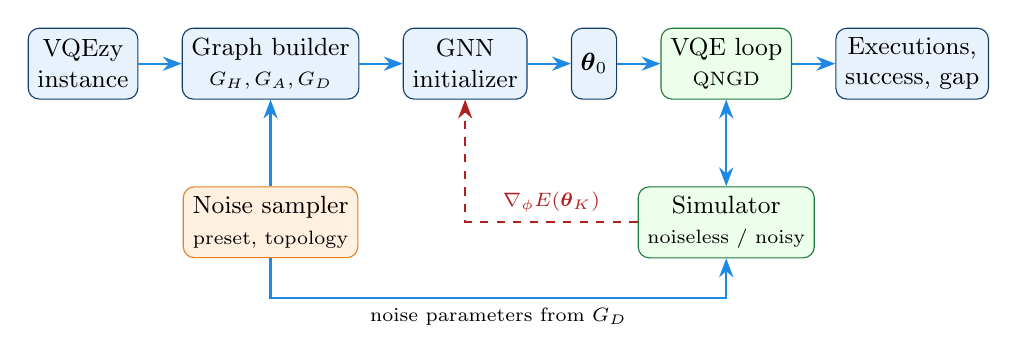
\begin{tikzpicture}[node distance=1.1cm and 0.55cm]
    \node[box] (inst) {VQEzy\\instance};
    \node[box,right=of inst] (gr) {Graph builder\\\scriptsize $G_H,G_A,G_D$};
    \node[box,right=of gr] (gnn) {GNN\\initializer};
    \node[box,right=of gnn] (th) {$\boldsymbol\theta_0$};
    \node[qbox,right=of th] (vqe) {VQE loop\\\scriptsize QNGD};
    \node[box,right=of vqe] (met) {Executions,\\success, gap};
    \node[nbox,below=of gr] (ns) {Noise sampler\\\scriptsize preset, topology};
    \node[qbox,below=of vqe] (sim) {Simulator\\\scriptsize noiseless / noisy};
    \draw[arrow] (inst)--(gr); \draw[arrow] (ns)--(gr); \draw[arrow] (gr)--(gnn);
    \draw[arrow] (gnn)--(th); \draw[arrow] (th)--(vqe); \draw[arrow] (vqe)--(met);
    \draw[{Stealth[length=2.4mm]}-{Stealth[length=2.4mm]},thick,draw=AccentBlue] (vqe)--(sim);
    \draw[arrow] (ns.south)--++(0,-0.5)-| node[pos=0.25,below,font=\scriptsize]{noise parameters from $G_D$} (sim.south);
    \draw[arrow,dashed,draw=BadRed] (sim.west) -| node[pos=0.25,above,font=\scriptsize,text=BadRed]{$\nabla_\phi E(\boldsymbol\theta_K)$} (gnn.south);
  \end{tikzpicture}

  \vspace{0.3cm}
  \small Dashed red: label-free training signal, the gradient of the energy after $K$ unrolled optimizer steps.
\end{frame}

% 6. Modules
\begin{frame}{System Modules}
  \begin{columns}[T,onlytextwidth]
    \column{0.55\textwidth}
    \begin{enumerate}
      \item \textbf{M1 Data \& Graphs:} VQEzy $\rightarrow$ $G_H,G_A,G_D$; fixed splits; noise-varied copy
      \item \textbf{M2 Simulation \& Noise:} PennyLane + own GPU density-matrix simulator
      \item \textbf{M3 GNN Initializer:} 3 GAT encoders, cross-attention, decoder
      \item \textbf{M4 Label-free Training:} unrolled GD / QNGD objectives
      \item \textbf{M5 VQE \& Evaluation:} Adam, QNGD, circuit accounting, scoring
    \end{enumerate}
    \column{0.42\textwidth}
    \centering
    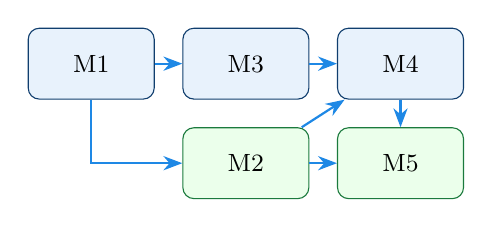
\begin{tikzpicture}[node distance=0.35cm and 0.35cm,every node/.style={font=\scriptsize}]
      \node[box,minimum width=1.6cm] (m1) {M1};
      \node[box,minimum width=1.6cm,right=of m1] (m3) {M3};
      \node[box,minimum width=1.6cm,right=of m3] (m4) {M4};
      \node[qbox,minimum width=1.6cm,below=of m3] (m2) {M2};
      \node[qbox,minimum width=1.6cm,right=of m2] (m5) {M5};
      \draw[arrow] (m1)--(m3); \draw[arrow] (m3)--(m4); \draw[arrow] (m1)|-(m2);
      \draw[arrow] (m2)--(m4); \draw[arrow] (m2)--(m5); \draw[arrow] (m4)--(m5);
    \end{tikzpicture}
  \end{columns}
\end{frame}

% 7. Methodology
\begin{frame}{Methodology -- the Study Ladder}
  \begin{columns}[T,onlytextwidth]
    \column{0.62\textwidth}
    \centering
    \resizebox{\linewidth}{!}{%
    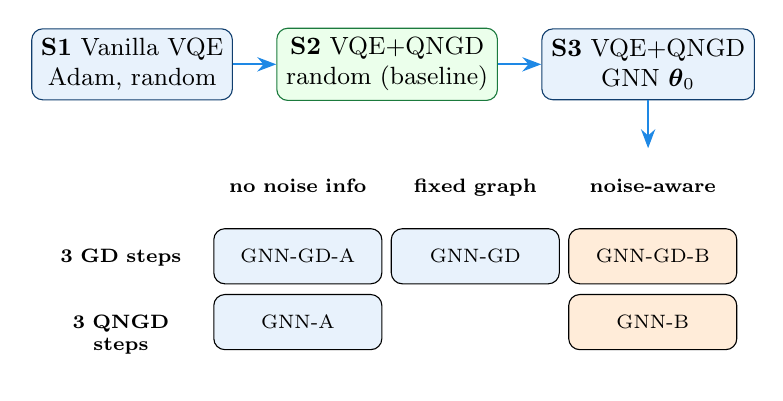
\begin{tikzpicture}[node distance=0.3cm and 0.55cm,every node/.style={font=\scriptsize}]
      \node[box,minimum width=2.2cm] (s1) {\textbf{S1} Vanilla VQE\\Adam, random};
      \node[qbox,minimum width=2.2cm,right=of s1] (s2) {\textbf{S2} VQE+QNGD\\random (baseline)};
      \node[box,minimum width=2.2cm,right=of s2] (s3) {\textbf{S3} VQE+QNGD\\GNN $\boldsymbol\theta_0$};
      \draw[arrow] (s1)--(s2); \draw[arrow] (s2)--(s3);
      \matrix (m) [below=0.6cm of s2.south,anchor=north,matrix of nodes,nodes in empty cells,
        column sep=3pt,row sep=3pt,ampersand replacement=\&,
        nodes={draw,rounded corners,minimum height=0.7cm,text width=1.9cm,align=center,font=\scriptsize}]
      {
        |[draw=none]| \& |[draw=none]| \textbf{no noise info} \& |[draw=none]| \textbf{fixed graph} \& |[draw=none]| \textbf{noise-aware} \\
        |[draw=none]| \textbf{3 GD steps}   \& |[fill=LightBlue]| GNN-GD-A \& |[fill=LightBlue]| GNN-GD \& |[fill=orange!15]| GNN-GD-B \\
        |[draw=none]| \textbf{3 QNGD steps} \& |[fill=LightBlue]| GNN-A    \& |[draw=none]|               \& |[fill=orange!15]| GNN-B \\
      };
      \draw[arrow] (s3.south)--(s3.south |- m.north);
    \end{tikzpicture}}
    \column{0.35\textwidth}
    \begin{block}{Evaluation Metrics}
      \begin{itemize}
        \item Circuit executions to target (device-level, \texttt{qml.Tracker})
        \item Success rate
        \item Final energy gap
        \item All of the above under noise
      \end{itemize}
    \end{block}
    \scriptsize 158 held-out instances, identical random starts and accounting for every study.
  \end{columns}
\end{frame}

% 8. Algorithm
\begin{frame}{Core Algorithm -- Label-free Unrolled Training}
  \begin{block}{Algorithm: train $f_\phi$ through the optimizer}
    \begin{enumerate}
      \item Build $G_H,G_A,G_D$ for a training instance; predict $\boldsymbol\theta_0=f_\phi(G_H,G_A,G_D)$
      \item Simulate $K=3$ optimizer steps (noisy if noise-aware):
            $\;\boldsymbol\theta_{k+1}=\boldsymbol\theta_k-\eta\,G_k\nabla E(\boldsymbol\theta_k)$,
            \quad $G_k=\begin{cases} I & \text{GD},\ \eta=0.1\\ F(\boldsymbol\theta_k)^{+} & \text{QNGD},\ \eta=0.02\end{cases}$
      \item Loss $\mathcal{L}=E(\boldsymbol\theta_K)$; back-propagate through every step (incl.\ $F^{+}$)
      \item Update $\phi$ with Adam; repeat over instances and epochs
    \end{enumerate}
  \end{block}
  \small MAML-style objective: the start is judged by \emph{where the optimizer gets to}, not by its own energy
  (minimizing $E(\boldsymbol\theta_0)$ gave flat, slow starts).
\end{frame}

% 9. Noise model
\begin{frame}{Graph-driven Noise Model}
  \begin{columns}[T,onlytextwidth]
    \column{0.5\textwidth}
    \begin{itemize}\small
      \item Noise numbers come \textbf{from $G_D$ itself} $\Rightarrow$ input and simulated noise agree
      \item CZ: depolarizing $p_{cz}=1-(1-\bar p)^{1+6(d-1)}$ (SWAP routing on the coupling map)
      \item RX/RY: depolarizing, per-qubit error
      \item Each layer: amplitude damping from $T_1$
      \item Readout: equivalent depolarizing $p=1.5r$ (exact for Pauli terms)
      \item Presets low / medium / high $\times$ topologies linear / ring / grid
    \end{itemize}
    \column{0.47\textwidth}
    \centering
    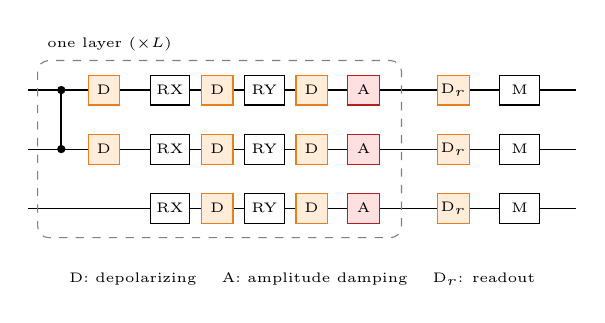
\begin{tikzpicture}[x=0.6cm,y=0.75cm,
       g/.style={draw,fill=white,minimum width=0.5cm,minimum height=0.38cm,font=\tiny,inner sep=1pt},
       c/.style={draw=NoiseOrange,fill=orange!15,minimum width=0.4cm,minimum height=0.38cm,font=\tiny,inner sep=1pt}]
      \foreach \q in {0,1,2} { \draw (0,-\q) -- (11.6,-\q); }
      \draw[dashed,gray,rounded corners] (0.2,0.5) rectangle (7.9,-2.5);
      \node[font=\tiny,anchor=south west] at (0.2,0.5) {one layer ($\times L$)};
      \draw[thick] (0.7,0)--(0.7,-1); \fill (0.7,0) circle (1.5pt); \fill (0.7,-1) circle (1.5pt);
      \node[c] at (1.6,0){D}; \node[c] at (1.6,-1){D};
      \foreach \q in {0,1,2} {
        \node[g] at (3.0,-\q){RX}; \node[c] at (4.0,-\q){D};
        \node[g] at (5.0,-\q){RY}; \node[c] at (6.0,-\q){D};
        \node[c,fill=red!12,draw=BadRed] at (7.1,-\q){A};
        \node[c] at (9.0,-\q){D$_r$}; \node[g] at (10.4,-\q){M};
      }
      \node[font=\tiny,align=center] at (5.8,-3.2){D: depolarizing \quad A: amplitude damping \quad D$_r$: readout};
    \end{tikzpicture}
  \end{columns}
\end{frame}

% 10. Implementation snapshot (replaces screenshots)
\begin{frame}[fragile]{Implementation Snapshot -- Differentiable QNGD Simulator}
  \begin{columns}[T,onlytextwidth]
    \column{0.52\textwidth}
\begin{lstlisting}[language=Python]
def qngd_unroll(self, theta0, K, eta):
    theta, energies = theta0, []
    for _ in range(K):
        e, pre = self.run(theta)   # density matrices
        energies.append(e)
        g = autograd.grad(e.sum(), theta,
                          create_graph=True)[0]
        F = self.metric_tensor(pre) # block-diag
        theta = theta - eta * (pinv(F) @ g)
    energies.append(self.energy(theta))
    return stack(energies, 1), theta
\end{lstlisting}
    \column{0.45\textwidth}
    \begin{block}{Validated against PennyLane}
      \scriptsize
      \begin{tabular}{@{}lr@{}}
        Noiseless energy & $4\!\times\!10^{-16}$\\
        Noisy energy (\texttt{default.mixed}) & $9\!\times\!10^{-12}$\\
        Noisy QNGD steps & $1\!\times\!10^{-13}$\\
        Meta-gradient vs.\ finite diff. & $3\!\times\!10^{-8}$\\
      \end{tabular}
    \end{block}
    \scriptsize Batched on an RTX A5000: noisy training $\approx$5$\times$ faster than the earlier CPU pipeline.
  \end{columns}
\end{frame}

% 11. Implementation status
\begin{frame}{Implementation Status}
  \small
  \begin{tabularx}{\textwidth}{X>{\centering\arraybackslash}p{2.2cm}X}
    \toprule
    \textbf{Modules} & \textbf{Status} & \textbf{Evidence / Remarks} \\
    \midrule
    M1 Data \& graphs & Completed & 1000/150/158 split; noise-varied copy (9 preset$\times$topology) \\
    M2 Simulation \& noise & Completed & GPU density-matrix simulator, validated to $10^{-12}$ \\
    M3 GNN initializer & Completed & 3 encoders + cross-attention; with/without noise branch \\
    M4 Training & Completed & 5 variants (GD / QNGD $\times$ noise awareness) + pilot \\
    M5 Evaluation & Completed & S1, S2, S3 noiseless and noisy \\
    Geometry head $\hat F_0$, QAOA ablation & Planned & After seed study \\
    \bottomrule
  \end{tabularx}
\end{frame}

% 12. Results S1 vs S2
\begin{frame}{Results 1 -- Vanilla VQE vs.\ VQE+QNGD (same random starts)}
  \begin{columns}[T,onlytextwidth]
    \column{0.56\textwidth}
    \centering
    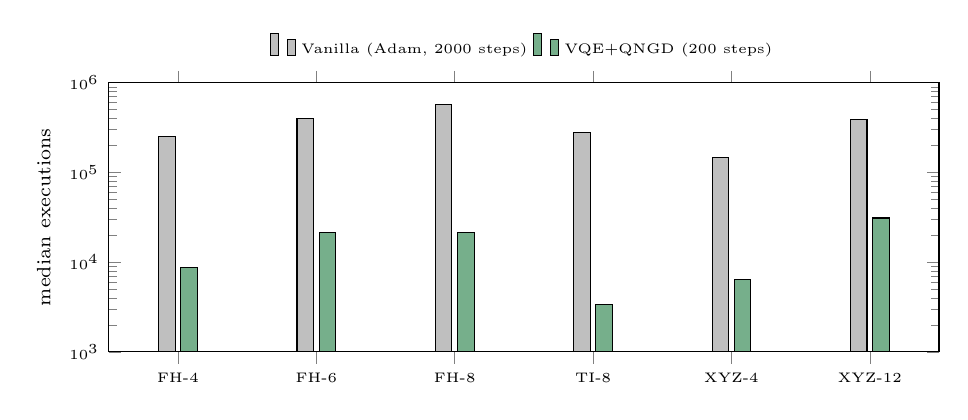
\begin{tikzpicture}
    \begin{axis}[ybar, ymode=log, log origin=infty, width=\linewidth, height=5.0cm, bar width=6pt,
      ylabel={\scriptsize median executions}, symbolic x coords={FH-4,FH-6,FH-8,TI-8,XYZ-4,XYZ-12},
      xtick=data, x tick label style={font=\tiny}, y tick label style={font=\tiny},
      legend style={font=\tiny,at={(0.5,1.05)},anchor=south,legend columns=2,draw=none},
      ymin=1000, ymax=1000000, enlarge x limits=0.1]
    \addplot[fill=gray!50] coordinates {(FH-4,253275) (FH-6,395430) (FH-8,569725) (TI-8,280800) (XYZ-4,145778) (XYZ-12,391541)};
    \addplot[fill=GoodGreen!60] coordinates {(FH-4,8663) (FH-6,21627) (FH-8,21266) (TI-8,3408) (XYZ-4,6431) (XYZ-12,31066)};
    \legend{{Vanilla (Adam{,} 2000 steps)\quad},{VQE+QNGD (200 steps)}}
    \end{axis}
    \end{tikzpicture}
    \column{0.42\textwidth}
    \begin{block}{Key Findings}
      \begin{itemize}\small
        \item Success: \textbf{54\% $\rightarrow$ 82\%}
        \item Executions when both succeed: \textbf{$\approx$2\%} of vanilla
        \item Total executions: \up{94\% fewer}
        \item QNGD cheaper in \textbf{387/407} paired runs
      \end{itemize}
    \end{block}
    \scriptsize Vanilla uses VQEzy's Adam ($\eta=10^{-3}$), charged parameter-shift cost per step.
  \end{columns}
\end{frame}

% 13. Results noiseless
\begin{frame}{Results 2 -- GNN Initialization on Top of QNGD (Noiseless)}
  \centering\small
  Circuit executions saved vs.\ VQE+QNGD from random starts (158 test instances)\\[2mm]
  \begin{tabular}{lccccc}
    \toprule
    Group & GNN-GD & GNN-GD-A & GNN-GD-B & GNN-A & GNN-B \\
    \midrule
    FH-4   & \up{+15.4\%} & \dn{$-$38.9\%} & \dn{$-$65.3\%} & \dn{$-$26.8\%} & \dn{$-$67.5\%} \\
    FH-8   & \dn{$-$7.6\%} & \dn{$-$71.8\%} & \dn{$-$68.3\%} & \dn{$-$64.9\%} & \dn{$-$77.7\%} \\
    TI-8   & \up{+65.1\%} & \up{+53.2\%} & \dn{$-$34.1\%} & \up{+8.5\%} & \dn{$-$8.3\%} \\
    XYZ-12 (unseen) & \up{+24.3\%} & \up{+35.3\%} & \up{+41.6\%} & \up{+47.5\%} & \up{+7.7\%} \\
    \midrule
    \textbf{All} & \up{+5.8\%} & \dn{$-$29.7\%} & \dn{$-$43.7\%} & \dn{$-$22.8\%} & \dn{$-$44.8\%} \\
    \bottomrule
  \end{tabular}\\[3mm]
  \raggedright
  \begin{itemize}\small
    \item Only \textbf{GNN-GD} beats the baseline without noise; all variants \textbf{generalize to 12 qubits}
    \item Fermi--Hubbard (FH) is hard for every initializer
  \end{itemize}
\end{frame}

% 14. Results noisy
\begin{frame}{Results 3 -- Under Device Noise}
  \begin{columns}[T,onlytextwidth]
    \column{0.55\textwidth}
    \centering\scriptsize
    Executions saved vs.\ random (150 noisy instances)\\[1mm]
    \begin{tabular}{lccc}
      \toprule
      Model & All & High noise & Ising \\
      \midrule
      GNN-GD   & \dn{$-$11.4\%} & \dn{$-$6.8\%} & \dn{0/30 reached} \\
      GNN-GD-A & \dn{$-$15.8\%} & \dn{$-$7.0\%} & \dn{0/30 reached} \\
      GNN-GD-B & \up{+12.8\%} & \up{+13.8\%} & \up{+92\%} \\
      GNN-A    & \up{+15.1\%} & \up{+13.3\%} & \up{+92\%} \\
      GNN-B    & \up{+14.9\%} & \up{+19.8\%} & \up{+94\%} \\
      \bottomrule
    \end{tabular}
    \column{0.43\textwidth}
    \begin{block}{Key Findings}
      \begin{itemize}\scriptsize
        \item Noiseless-trained GD models are \textbf{noise-blind} (output changes $<10^{-3}$ rad with $G_D$)
        \item \textbf{Training under noise} turns GD recipe from \dn{$-$15.8\%} into \up{+12.8\%}
              (wins 70 vs.\ 16 instances)
        \item QNGD-trained models are robust even without noise training
        \item Noise awareness pays off most at \textbf{high noise} (GNN-B \up{+19.8\%})
      \end{itemize}
    \end{block}
  \end{columns}
\end{frame}

% 15. Summary chart
\begin{frame}{Results Summary -- No Single Winner Yet}
  \begin{columns}[T,onlytextwidth]
    \column{0.6\textwidth}
    \centering
    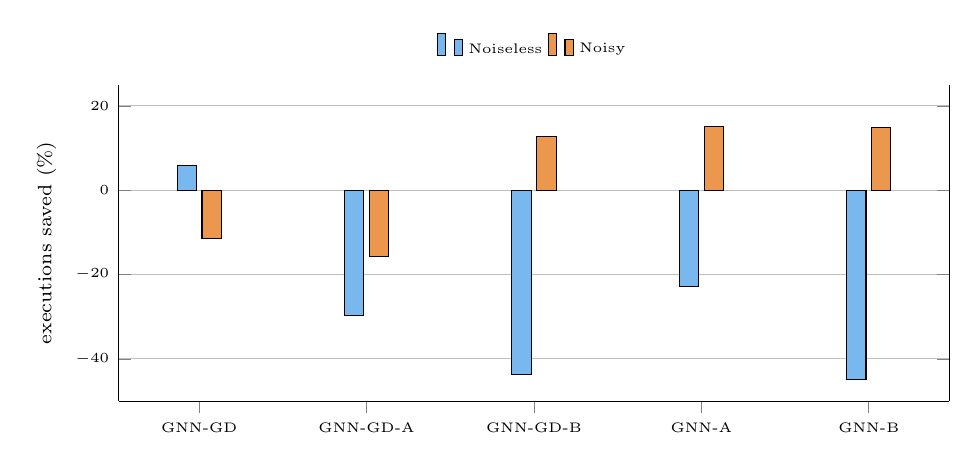
\begin{tikzpicture}
    \begin{axis}[ybar, width=\linewidth, height=5.6cm, bar width=7pt,
      ylabel={\scriptsize executions saved (\%)},
      symbolic x coords={GNN-GD,GNN-GD-A,GNN-GD-B,GNN-A,GNN-B}, xtick=data,
      x tick label style={font=\tiny}, y tick label style={font=\tiny},
      ymin=-50, ymax=25, ymajorgrids, axis x line*=bottom,
      legend style={font=\tiny,at={(0.5,1.05)},anchor=south,legend columns=2,draw=none},
      enlarge x limits=0.12]
    \addplot[fill=AccentBlue!60] coordinates {(GNN-GD,5.8) (GNN-GD-A,-29.7) (GNN-GD-B,-43.7) (GNN-A,-22.8) (GNN-B,-44.8)};
    \addplot[fill=NoiseOrange!80] coordinates {(GNN-GD,-11.4) (GNN-GD-A,-15.8) (GNN-GD-B,12.8) (GNN-A,15.1) (GNN-B,14.9)};
    \legend{Noiseless\quad,Noisy}
    \end{axis}
    \end{tikzpicture}
    \column{0.37\textwidth}
    \begin{block}{Interpretation}
      \begin{itemize}\scriptsize
        \item The \textbf{optimizer} gives the big win (94\%)
        \item The \textbf{training objective} decides what a ``good start'' is
        \item 3-step QNGD training $\Rightarrow$ fast early drop, then stall (\emph{short-horizon bias})
        \item Best model depends on the \textbf{noise regime}
      \end{itemize}
    \end{block}
  \end{columns}
\end{frame}

% 16. Limitations and next steps
\begin{frame}{Limitations and Next Steps}
  \begin{columns}[T,onlytextwidth]
    \column{0.48\textwidth}
    \begin{alertblock}{Limitations}
      \begin{itemize}\scriptsize
        \item One training seed per model; gaps of a few \% not significant
        \item GD replication gap: GNN-GD-A $-$29.7\% vs.\ GNN-GD +5.8\% (noiseless)
        \item Noise-aware models never saw a zero-noise graph
        \item Synthetic noise presets; relative energy target
        \item VQEzy's stored runs are 1-layer (found in this work)
      \end{itemize}
    \end{alertblock}
    \column{0.48\textwidth}
    \begin{block}{Next Steps}
      \begin{enumerate}\scriptsize
        \item Seed study: 3 seeds per model, best + last epoch
        \item Add a zero-noise preset to noise-aware training
        \item Normalized longer-horizon objective
        \item Geometry head $\hat F_0$ to cut QNGD's metric cost
        \item QAOA ablation and Qracle-style baseline
      \end{enumerate}
    \end{block}
  \end{columns}
\end{frame}

% 17. Responsibilities
\begin{frame}{Team Responsibilities}
  \small
  \begin{tabularx}{\textwidth}{>{\bfseries}p{3.6cm}X p{2.3cm}}
    \toprule
    Team Member & Responsibilities & Current Status \\
    \midrule
    R.K.\ Barath & [Responsibilities] & [Status] \\
    Nithyasree.K & [Responsibilities] & [Status] \\
    Madhangi Karimanal & [Responsibilities] & [Status] \\
    \bottomrule
  \end{tabularx}
\end{frame}

% 18. References
\begin{frame}[allowframebreaks]{References}
  \footnotesize
  \begin{thebibliography}{9}
    \bibitem{peruzzo} A. Peruzzo \emph{et al.}, ``A variational eigenvalue solver on a photonic quantum processor,'' \emph{Nature Communications}, vol.~5, 4213, 2014. DOI: 10.1038/ncomms5213.
    \bibitem{stokes} J. Stokes, J. Izaac, N. Killoran, and G. Carleo, ``Quantum natural gradient,'' \emph{Quantum}, vol.~4, p.~269, 2020. DOI: 10.22331/q-2020-05-25-269.
    \bibitem{qracle} C. Zhang, L. Jiang, and F. Chen, ``Qracle: A graph-neural-network-based parameter initializer for variational quantum eigensolvers,'' \emph{Proc. IEEE QCE}, 2025, pp.~197--207.
    \bibitem{vqezy} ``VQEzy: A dataset for variational quantum eigensolver parameter initialization,'' arXiv:2509.17322, 2025.
    \bibitem{metavqe} A. Cervera-Lierta, J. S. Kottmann, and A. Aspuru-Guzik, ``Meta-variational quantum eigensolver,'' \emph{PRX Quantum}, vol.~2, 020329, 2021. DOI: 10.1103/PRXQuantum.2.020329.
    \bibitem{maml} C. Finn, P. Abbeel, and S. Levine, ``Model-agnostic meta-learning for fast adaptation of deep networks,'' \emph{ICML}, 2017. arXiv:1703.03400.
    \bibitem{wu} Y. Wu, M. Ren, R. Liao, and R. Grosse, ``Understanding short-horizon bias in stochastic meta-optimization,'' \emph{ICLR}, 2018. arXiv:1803.02021.
    \bibitem{mcclean} J. R. McClean \emph{et al.}, ``Barren plateaus in quantum neural network training landscapes,'' \emph{Nature Communications}, vol.~9, 4812, 2018. DOI: 10.1038/s41467-018-07090-4.
    \bibitem{gat} P. Veli\v{c}kovi\'{c} \emph{et al.}, ``Graph attention networks,'' \emph{ICLR}, 2018. arXiv:1710.10903.
    \bibitem{pennylane} V. Bergholm \emph{et al.}, ``PennyLane: Automatic differentiation of hybrid quantum-classical computations,'' arXiv:1811.04968, 2018.
  \end{thebibliography}
\end{frame}

% 19. Thank you
\begin{frame}[plain]
  \centering
  \vfill
  {\usebeamerfont{title}\color{UniversityBlue}\Huge Thank You}\par
  \vspace{0.5cm}
  {\Large Questions and Discussion}\par
  \vspace{0.8cm}
  \vfill
\end{frame}

\end{document}
